\chapter{Dynamisches Programmieren}

\section{Dominating Set}

  Sei ein Graph \(G = (V,E)\) gegeben. Wir nennen eine Menge \(D \subseteq V\) \defNotion{dominierend}, falls jeder Knoten in \(V \setminus D\) adjazent zu einem Knoten aus \(D\) ist.

  Ein brute-force-Algorithmus für das kleinste dominating set läuft in \(O^*(2^n)\) durch Ausprobieren aller Teilmengen von \(V\). Zur Verbesserung dieser Laufzeit betrachten wir nicht erweiterbare unabhängige Mengen (NEUM) und verwenden dynamische Progammierung. Wir beobachten, dass sich eine NEUM effizient ermitteln lässt und jede NEUM dominierend ist.

  \paragraph{Idee.} Zunächst bestimmen wir ein NEUM \(I\). Falls dieses klein ist, können wir alle Knotenmengen \(D\) mit \(|D| \leq |I|\) ausprobieren. Falls \(I\) groß ist, wenden wir das folgende Verfahren an.

  \begin{lemma}
    Sei \(G\) ein Graph und \(I\) ein zugehöriges NEUM. Dann lässt sich eine kleinste dominierende Menge in \(O^*(2^{n-|I|})\) ermitteln.
  \end{lemma}

  Beweis fehlt.

%   \begin{proof}
%     Wir definieren für Teilmengen \(D \subseteq V\) die Menge \(J_D \isDefinedBy D \cap J\) und \[\gamma \isDefinedBy \min \{ |D| : D \text{ dominiert } G \}.\] Dann ist die Menge \(I_D \isDefinedBy I \setminus N(J_D) = I \setminus N(J \cap D)\) in \(D\) enthalten, denn ein \(v \in I \setminus N(J \cap D)\) liegt in \(I\), jedoch nicht in der Nachbarschaft von \(J \cap D\). Damit wird \(v\) nicht von \(J \cap D\) dominiert. Da aber \(D\) eine dominierende Menge ist, muss \(v\) von \(I \cap D\) dominiert werden. .... \(v\) liegt nicht in \(N(J \cap D)\) und nicht in \(N(I \cap D)\), also \(v \notin N(D)\). Da \(v \notin N(D)\) und \(D\) dominierende Menge, gilt also \(v \in D\).
%   \end{proof}  

  \marginpar{15.5.12}
  
  \begin{lemma}
    Sei \(\alpha \leq 1/2\). Dann gilt \[ \sum_{i=0}^{\alpha \cdot n} \binom{n}{i} = O^*( 2^{h(\alpha) \cdot n} ), \] wobei \(h(\alpha) = - \alpha \log_2 \alpha - (1-\alpha) \log_2(1 - \alpha)\).
  \end{lemma}
  
  \begin{figure}[h]
    \centering
    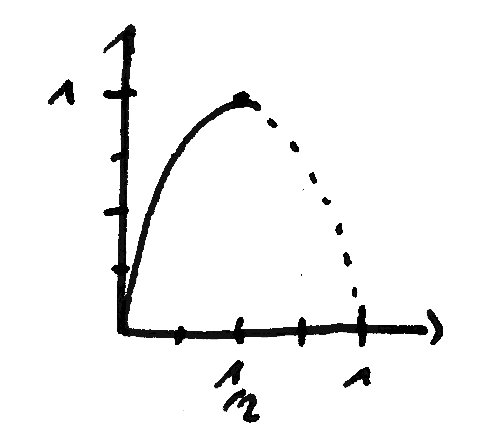
\includegraphics[width=.25\textwidth]{./Bilder/b01.jpg}
    % b01.jpg: 495x434 pixel, 72dpi, 17.46x15.31 cm, bb=0 0 495 434
    \caption{Graph des Binomialkoeffizienten}
  \end{figure}
  
  \begin{proof}
    Es ist \( \sum_{i=0}^{\alpha n} \leq n \binom{n}{\alpha n} = O^*( \binom{n}{\alpha n} ) \), denn die Binomialkoeffizienten \( \binom{a}{b} \) steigen für \(b \leq n/2\) monoton an. Per Definition gilt 
    \[
      \binom{n}{k} = \frac{n!}{k! (n-k)!}.
    \]
    Die Fakultät kann abgeschätzt werden durch \( \sqrt{2 \pi n} (n/e)^n \leq n! \leq 2 \sqrt{2 \pi n} (n/e)^n \), also ist \(n!\) proportional zu \((n/e)^n\). Daraus folgt, dass 
    \begin{eqnarray*}
      \binom{n}{\alpha n} &=& O^* \left( \frac{(n/e)^n}{(\alpha n/e)^{\alpha n} ( (1-\alpha)n/e)^{(1-\alpha) n}} \right) = O^* \left( \alpha^{-\alpha n} (1-\alpha)^{-(1-\alpha)n} \right) \\
      &=& O^* \left( 2^{-\alpha \log_2 \alpha n} \cdot 2^{-(1 - \alpha) \log_2(1-\alpha)n} \right),
    \end{eqnarray*}
    woraus die Behauptung folgt.
  \end{proof}
  
  \begin{theorem}
    Eine kleinste dominierende Menge lässt sich in \(O(1{,}7088^n)\) ermitteln.
  \end{theorem}
  
  \begin{proof}
    Zunächst bestimmen wir eine nicht-erweiterbare unabhänge Menge \(I\). 
    Falls \(|I| \leq \alpha n\), testen wir in \(O^*(2^{h(\alpha) n})\) alle Teilmengen \(D \subseteq V\) mit \(|D| \leq |I|\).
    Falls \(|I| > \alpha n\), wende Satz \ref{satz??} an und berechne kleinste dominierende Menge in \(O^*(2^{(1-\alpha)n})\). % Satz in dem O*(2^(n-|I|)) bewiesen wurde
    
    \begin{figure}[h]
      \centering
      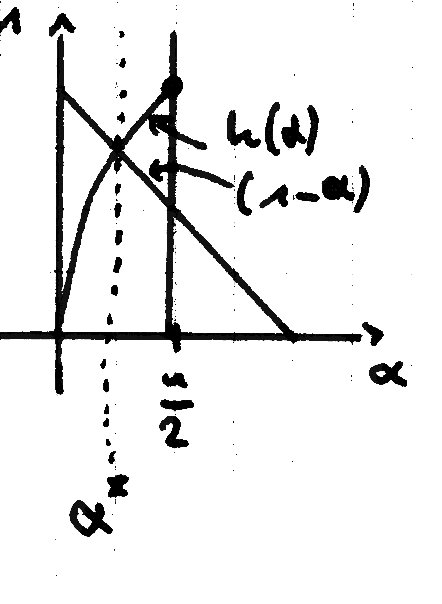
\includegraphics[width=.25\textwidth]{./Bilder/b02.jpg}
      % b02.jpg: 442x604 pixel, 72dpi, 15.59x21.31 cm, bb=0 0 442 604
      \caption{Bestimmung von \(\alpha^*\) als Maximum der zwei möglichen Funktionen}
    \end{figure}
    
    Aus der Skizze ergibt sich die Laufzeit als das Maximum der beiden dargestellten Funktionen bei \(\alpha^* \leq 0,22711\) bzw. \(O(2^{0,7729n}) = O(1,7088^n)\).
  \end{proof}
  
  Der schnellste derzeit bekannte Algorithmus für dieses Problem benötigt ca. \(O(1,5^n)\) und stammt aus 2010.



